\begin{center}
	\textit{ \textbf{\Large{La Regression}  } }
\end{center}
\paragraph{}
la régression est une technique consistant à prédire la sortie  d'une    observation en partant d'un certain nombre des variables  en entrée.

on part d'un certain nombre des données  d'apprentissage ou  d'un training set 
avec :

m :  nombres des données d'apprentissage

${x}_{1}$ ,${x}_{2}$,${x}_{3}$ .... ${x}_{n}$ : les variables d'entrées(qui peuvent varier de 1 (pour la régression linéaire avec une seule variable ) à n pour plusieurs variables  )

y : la variable  de sortie
on notera le (${x}_{1}$,${x}_{2}$,${x}_{3}$ .... ${x}_{n}$, y) : un exemple d'apprentissage
et

(${x}_{1}^{i}$,${x}_{2}^{i}$,${x}_{3}^{i}$......${x}_{n}^{i}$,${y}^{i}$)  un exemple choisie le ème exemple d'apprentissage avec  i comme index sur nos données.

l'objectif de la régression c'est de trouver la fonction qui minimise l'erreur entre les valeurs de la fonction aux points d'apprentissage et la valeur de sortie dans les données d'apprentissage  et ensuite l'utilise pour effectuer des prédiction.
cette fonction on l'appellera notre hypothèse qui sera une droite ou un polynôme selon qu'on utilise la régression linéaire ou polynomiale 
notre hypothèse se présentera de la manière suivante :

\textbf{\emph{1 ère cas régression avec un seule variable: }} 

par exemple on tente de prédire le prix d'une maison en fonction de sa superficie

${h}_{\theta}\left(x\right)={\theta }_{0}+{\theta }_{1}x$

cela signifie que  y est une fonction linéaire de x avec ${\theta }_{i}$ des paramètres qu'on cherchera à déterminer .
on peut le remarque sur la figure suivante ou notre hypothèse est une droite :
\begin{figure}[ht]
	\centering
	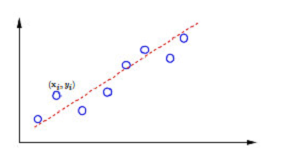
\includegraphics[width=0.5\textwidth]{fig/regressionLineaire1var.png}
	\caption[Short caption]{Régression Linéaire avec une variable}
	\label{fig:imageGraph}
\end{figure}

\textbf{\emph{2 ème cas régression avec plusieurs variables :}}

par exemple prédire le prix d'une maison cette fois en fonction de la superficie, du nombre des chambres ,et de l'année de construction

${h}_{\theta}\left(x\right)={\theta }_{0}{x}_{0}+{\theta }_{1}{x}_{1}+{\theta }_{2}{x}_{2}+{\theta }_{3}{x}_{3}+....{\theta }_{n}{x}_{n}$

\textbf{\emph{3 eme cas la regression polynomiale:}}

dans ce cas au lieu d'utiliser une droite on utilise un polynôme à n degree qui es donnée par:

${h}_{\theta}\left(x\right)={\theta }_{0}{x}_{0}+{\theta }_{1}{x}_{1}+{\theta }_{2}{x}_{2}^{2}+{\theta }_{3}{x}_{3}^{3}+....{\theta }_{n}{x}_{n}^{n}$
\begin{figure}[ht]
	\centering
	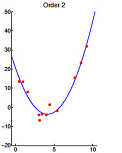
\includegraphics[width=0.5\textwidth]{fig/regressionPlokynome.png}
	\caption[Short caption]{Régression Polynomiale avec un polynôme de degré 2}
	\label{fig:imageGraph}
\end{figure}
le travail restant sera de trouver les paramètres ${\theta }_{i}$ pour notre fonction  ${h}_{\theta}\left(x\right)$ mais comment les trouver?

\textbf{\emph{Définition:}}
on appelle l'erreur de prédiction la valeur définie par   :

 $J\left({\theta }_{1},{\theta }_{2},.....{\theta }_{n}\right)=\frac{1}{2m}\sum _{=1}^{m}{\left[{h}_{\theta}\left({x}^{(i)}\right) - {y}^{(i)}\right]}^2$
 
 
 avec m : le nombre des nos données d'apprentissage
 
 les  ${\theta }_{i}$ sont les valeurs qui minimisent cette erreur sur toutes les données de notre apprentissage
 
 il existe différents techniques de minimisation de cette fonction entre autre :
 
  - L'annulation de la dérivée première (trouver les valeurs ${\theta }_{i}$ qui annulent notre dérivée première  )   cette méthode à pour inconvénient le fait qu'il convient pas pour les données d'apprentissage avec plusieurs attribues et plusieurs données. 
  - une autre méthode c'est la descente du gradient :
  celle ci consiste à effectuer plusieurs itérations sur les valeurs de  ${\theta }_{i}$ jusqu'à trouver celle qui minimise l'erreur (jusqu'à ce qu'il converge vers zéro)
  
  voici l'algorithme utilisée :
\ref{Algo1}
\begin{algorithm}[ht]
	\caption{Algorithme de la descente du gradient }
	\label{Algo1}
	\begin{algorithmic}
		\State ${\theta }_{i} \leftarrow 0$
		\While{J ne converge pas}\Comment{faire pour chaque tuple }
		\State ${\theta }_{i} \leftarrow  {\theta }_{i} - \alpha \frac{\partial }{\partial {{\theta }_{i}}}J\left({\theta }_{1},{\theta }_{2},.....{\theta }_{n}\right)$
		\EndWhile
	\end{algorithmic}
   \end{algorithm}
  
  avec $\alpha$ : learning rate qui est compris entre [0,001;0,1] il sert à réguler notre algorithme
  
  s'il est trop grand $\theta$ ne converge pas
  s'il est trop petit $\theta$ converge après plusieurs itérations. 
  Dans la plupart des cas J converge après un nombre d'itérations élevé
  comme on peut le remarqué sur la figure suivante :
  \begin{figure}[ht]
  	\centering
  	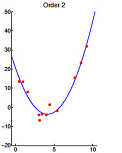
\includegraphics[width=0.5\textwidth]{fig/regressionPlokynome.png}
  	\caption[Short caption]{Variation de J en fonction du nombre des itérations}
  	\label{fig:imageGraph}
  \end{figure}
   
  
  NB :  La Normalisation
  
  Dans la pratique on peut avoir plusieurs données qui ne sont pas dans la même echelle
  
  par ex:
   surface ${x}_{1}$ : compris entre 30 -- 400 ${m}^2$
   nombres des chambres ${x}_{1}$ : 1-10
   
   et cela peut présenter un problème de convergence et ainsi empêcher les ${\theta }_{i}$ de converger rapidement .
   pour limiter ce problème on effectue un normalisation elle consister à remplacer les ${x}_{i}$ pour chaque tuple par :
   
        ${x}_{j}^{i} =  \frac{{x}_{j}^{i}- {\mu({x}_{j})}}{{\sigma({x}_{j})}}$
        avec :
        
        ${\mu({x}_{j})}$ : la moyenne des termes  ${x}_{j}$ et 
        ${\sigma({x}_{j})}$ : la variance des termes  ${x}_{j}$ 
        